% Domain Adaptation in Computer Vision
%   Why DA is important --> Start with an example in medical imaging, add a picture to show everything
%   The amount of information determines the flavor: Types of Domain Adaptation (Unsupervised, source free...)
%   Domain Adaptation in Real-World Applications  ---> Probably not!

\textfig[t]{1}{Figures/domain_adaptation_example.pdf}{Brain MRI scans from three sites (UMC Utrecht, NUHS Singapore, and VU Amsterdam) with the FLAIR acquisition. Although all examples have been acquired with FLAIR acquisition, each site has different acquisition parameters, leading to visible differences in image properties. Images from the WMH dataset~\cite{wmh}.}{fig:domain_adaptation_example}

\section{Domain Adaptation}\label{sec:domain_adaptation}\index{domain adaptation}


\Cref{fig:domain_adaptation_example} shows brain MRI scans from three sites with the same acquisition type. At the same time, \Cref{fig:domain_adaptation_intensity} presents a quantification of the pixel intensity distribution per site normalized within that site. Both figures suggest that image values are not only dependent on the field of application\sidenote{Of course, the pixel distribution of road images acquired for self-driving cars and that of brain MRIs will be completely different.}, nor on the acquisition type, but also on the particular settings defined on-site. This poses a critical problem for computer vision: how to build models that bridge the domain shift\sidenote{See \Cref{subsec:da_intro}, where this term was introduced.}, \ie~that generalize data with the same semantic distribution but different features. For example, in \Cref{fig:domain_adaptation_example}, all three images have the same semantic information (brain MRIs with white matter hyperintensities), but the images' features are very different. We say in this case that the source domain\sidedef{Source Domain}{Initial domain in which a ML model is trained.} --- the initial domain on which the model is trained --- is different from the target domain\sidedef{Target Domain}{Domain to which a pre-trained model is applied.} --- the domain to which we are applying the model.

\textfig[t]{1}{Figures/domain_adaptation_intensity.pdf}{Quantification of pixel intensity differences across three sites of the WMH dataset~\cite{wmh}.}{fig:domain_adaptation_intensity}

In this section, we will explore how the field of Domain Adaptation (DA) is searching for the answer to the previous question. We will see that the answer depends on the amount of information in both the source and the target domains during training and how the complexity of the problem increases as this variable decreases.

\subsection{The Amount of Information Determines the Flavor}
Just as the presence or absence of labels categorizes the learning paradigms, it also categorizes the different types of domain adaptation. However, the presence of two domains introduces a certain degree of complexity. For instance, one may have no source domain images available, yet a few target labels and a substantial number of target images. When developing a domain adaptation model, it becomes crucial to ascertain the scenario at hand, as the techniques employed will vary. Nevertheless, all techniques and domain adaptation paradigms aim to construct a domain invariant representation or utilize information from the source domain in the target. 

\begin{figure}[t]
    \centering
    \FloatBarrier
    \sidecaption{Conceptual model of the learning paradigms, wherein the number of unlabeled source images and labeled and unlabeled target images serve
as the axes. Not having target labels is common, as it otherwise becomes either semi-supervised or supervised learning. Two scenarios only differ in the number of target images (source-free and test-time domain adaptation [SFDA and TTDA, respectively]) and one has no target images available (self-supervised learning).\label{fig:da_cube}
}
    \resizebox{\columnwidth}{!}{%



\tikzset{every picture/.style={line width=0.75pt}} %set default line width to 0.75pt        

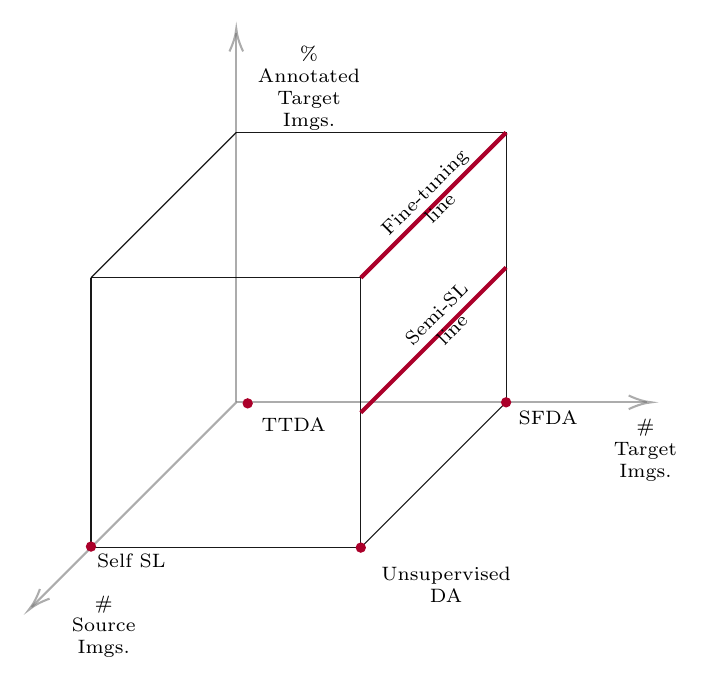
\begin{tikzpicture}[x=0.75pt,y=0.75pt,yscale=-1,xscale=1]
%uncomment if require: \path (0,402); %set diagram left start at 0, and has height of 402

%Straight Lines [id:da6807006831993536] 
\draw [color={rgb, 255:red, 117; green, 117; blue, 117 }  ,draw opacity=0.6 ][line width=0.75]    (270,210) -- (270,32) ;
\draw [shift={(270,30)}, rotate = 90] [color={rgb, 255:red, 117; green, 117; blue, 117 }  ,draw opacity=0.6 ][line width=0.75]    (10.93,-3.29) .. controls (6.95,-1.4) and (3.31,-0.3) .. (0,0) .. controls (3.31,0.3) and (6.95,1.4) .. (10.93,3.29)   ;
%Straight Lines [id:da5295149315723777] 
\draw [color={rgb, 255:red, 117; green, 117; blue, 117 }  ,draw opacity=0.6 ][line width=0.75]    (270,210) -- (468,210) ;
\draw [shift={(470,210)}, rotate = 180] [color={rgb, 255:red, 117; green, 117; blue, 117 }  ,draw opacity=0.6 ][line width=0.75]    (10.93,-3.29) .. controls (6.95,-1.4) and (3.31,-0.3) .. (0,0) .. controls (3.31,0.3) and (6.95,1.4) .. (10.93,3.29)   ;
%Straight Lines [id:da534666056608414] 
\draw [color={rgb, 255:red, 117; green, 117; blue, 117 }  ,draw opacity=0.6 ][line width=0.75]    (270,210) -- (171.41,308.59) ;
\draw [shift={(170,310)}, rotate = 315] [color={rgb, 255:red, 117; green, 117; blue, 117 }  ,draw opacity=0.6 ][line width=0.75]    (10.93,-3.29) .. controls (6.95,-1.4) and (3.31,-0.3) .. (0,0) .. controls (3.31,0.3) and (6.95,1.4) .. (10.93,3.29)   ;
%Straight Lines [id:da0025027309814475984] 
\draw [color={rgb, 255:red, 0; green, 0; blue, 0 }  ,draw opacity=0.9 ]   (270,80) -- (400,80) ;
%Straight Lines [id:da3170933147390458] 
\draw [color={rgb, 255:red, 0; green, 0; blue, 0 }  ,draw opacity=0.9 ]   (400,80) -- (400,210) ;
%Straight Lines [id:da8084774068453204] 
\draw [color={rgb, 255:red, 0; green, 0; blue, 0 }  ,draw opacity=0.9 ]   (400,210) -- (330,280) ;
%Straight Lines [id:da14868444296828032] 
\draw [color={rgb, 255:red, 0; green, 0; blue, 0 }  ,draw opacity=0.9 ]   (200,280) -- (330,280) ;
%Straight Lines [id:da9908929804494571] 
\draw [color={rgb, 255:red, 0; green, 0; blue, 0 }  ,draw opacity=0.9 ]   (330,150) -- (330,280) ;
%Straight Lines [id:da0019316496763430724] 
\draw [color={rgb, 255:red, 0; green, 0; blue, 0 }  ,draw opacity=0.9 ]   (200,150) -- (200,280) ;
%Straight Lines [id:da7518926340375516] 
\draw [color={rgb, 255:red, 0; green, 0; blue, 0 }  ,draw opacity=0.9 ]   (200,150) -- (330,150) ;
%Straight Lines [id:da3769124480681334] 
\draw [color={rgb, 255:red, 0; green, 0; blue, 0 }  ,draw opacity=0.9 ]   (270,80) -- (200,150) ;
%Straight Lines [id:da5228594606876449] 
\draw [color={rgb, 255:red, 171; green, 0; blue, 42 }  ,draw opacity=1 ][line width=1.5]    (400,145) -- (330,215) ;
%Straight Lines [id:da4767901038712239] 
\draw [color={rgb, 255:red, 171; green, 0; blue, 42 }  ,draw opacity=1 ][line width=1.5]    (400,80) -- (330,150) ;
%Shape: Circle [id:dp5300687249748464] 
\draw  [draw opacity=0][fill={rgb, 255:red, 171; green, 0; blue, 42 }  ,fill opacity=1 ] (327.5,280) .. controls (327.5,278.62) and (328.62,277.5) .. (330,277.5) .. controls (331.38,277.5) and (332.5,278.62) .. (332.5,280) .. controls (332.5,281.38) and (331.38,282.5) .. (330,282.5) .. controls (328.62,282.5) and (327.5,281.38) .. (327.5,280) -- cycle ;
%Shape: Circle [id:dp9711792189769151] 
\draw  [draw opacity=0][fill={rgb, 255:red, 171; green, 0; blue, 42 }  ,fill opacity=1 ] (273,210.5) .. controls (273,209.12) and (274.12,208) .. (275.5,208) .. controls (276.88,208) and (278,209.12) .. (278,210.5) .. controls (278,211.88) and (276.88,213) .. (275.5,213) .. controls (274.12,213) and (273,211.88) .. (273,210.5) -- cycle ;
%Shape: Circle [id:dp6127433690927064] 
\draw  [draw opacity=0][fill={rgb, 255:red, 171; green, 0; blue, 42 }  ,fill opacity=1 ] (397.5,210) .. controls (397.5,208.62) and (398.62,207.5) .. (400,207.5) .. controls (401.38,207.5) and (402.5,208.62) .. (402.5,210) .. controls (402.5,211.38) and (401.38,212.5) .. (400,212.5) .. controls (398.62,212.5) and (397.5,211.38) .. (397.5,210) -- cycle ;
%Shape: Circle [id:dp8193525877009633] 
\draw  [draw opacity=0][fill={rgb, 255:red, 171; green, 0; blue, 42 }  ,fill opacity=1 ] (197.5,279.5) .. controls (197.5,278.12) and (198.62,277) .. (200,277) .. controls (201.38,277) and (202.5,278.12) .. (202.5,279.5) .. controls (202.5,280.88) and (201.38,282) .. (200,282) .. controls (198.62,282) and (197.5,280.88) .. (197.5,279.5) -- cycle ;

% Text Node
\draw (275,37) node [anchor=north west][inner sep=0.75pt]  [font=\scriptsize] [align=left] {\begin{minipage}[lt]{43.21pt}\setlength\topsep{0pt}
\begin{center}
\% Annotated\\Target Imgs.
\end{center}

\end{minipage}};
% Text Node
\draw (447,217) node [anchor=north west][inner sep=0.75pt]  [font=\scriptsize] [align=left] {\begin{minipage}[lt]{28.38pt}\setlength\topsep{0pt}
\begin{center}
\# Target\\Imgs.
\end{center}

\end{minipage}};
% Text Node
\draw (184,302) node [anchor=north west][inner sep=0.75pt]  [font=\scriptsize] [align=left] {\begin{minipage}[lt]{31.29pt}\setlength\topsep{0pt}
\begin{center}
\# Source\\Imgs.
\end{center}

\end{minipage}};
% Text Node
\draw (331,288) node [anchor=north west][inner sep=0.75pt]  [font=\scriptsize] [align=left] {\begin{minipage}[lt]{58.26pt}\setlength\topsep{0pt}
\begin{center}
Unsupervised DA
\end{center}

\end{minipage}};
% Text Node
\draw (404.5,213) node [anchor=north west][inner sep=0.75pt]  [font=\scriptsize] [align=left] {\begin{minipage}[lt]{21.76pt}\setlength\topsep{0pt}
\begin{center}
SFDA
\end{center}

\end{minipage}};
% Text Node
\draw (342.12,185.25) node [anchor=north west][inner sep=0.75pt]  [font=\scriptsize,rotate=-315] [align=left] {\begin{minipage}[lt]{42.92pt}\setlength\topsep{0pt}
\begin{center}
Semi-SL line
\end{center}

\end{minipage}};
% Text Node
\draw (332.12,130.81) node [anchor=north west][inner sep=0.75pt]  [font=\scriptsize,rotate=-315] [align=left] {\begin{minipage}[lt]{51.53pt}\setlength\topsep{0pt}
\begin{center}
Fine-tuning line
\end{center}

\end{minipage}};
% Text Node
\draw (281,212) node [anchor=north west][inner sep=0.75pt]  [font=\scriptsize] [align=left] {\begin{minipage}[lt]{21.36pt}\setlength\topsep{0pt}
\begin{center}
TTDA
\end{center}

\end{minipage}};
% Text Node
\draw (201,282) node [anchor=north west][inner sep=0.75pt]  [font=\scriptsize] [align=left] {\begin{minipage}[lt]{25.74pt}\setlength\topsep{0pt}
\begin{center}
Self SL
\end{center}

\end{minipage}};


\end{tikzpicture}
}
\end{figure}

\Cref{fig:da_cube} depicts a conceptual model of the learning paradigms, wherein the number of unlabeled source images and labeled and unlabeled target images serve as the axes\sidenote{A representation of all the learning paradigms requires one more dimension. I had trouble representing four dimensions in a 2D paper, so I had to discard one of them.}. It can be observed that not having target labels is common, as it otherwise becomes either semi-supervised or supervised learning. Additionally, there are two scenarios that only differ in the number of target images (source-free and test-time domain adaptation) and one where no target images are available (self-supervised learning).

\begin{itemize}
    \item \textbf{Semi-Supervised DA} is very similar to traditional semi-supervised learning\sidenote{See \nameref{subsec:semi_self} in \Cref{sec:training_paradigms}.}. What defines this category is the presence of some labeled target images and a larger amount of unlabeled ones. Training strategies do not differ significantly from those used for semi-supervised learning, using the unlabeled samples for feature alignment and a regularization term that leverages the labeled samples.
    
    \item In \textbf{Unsupervised DA}, target labels are not present, and source images are often available with or without labels. This implies that the model can only learn the target domain features from feature alignment tasks, and regularization can be done with the source images.
    
    \item \textbf{Source-Free DA} (SFDA) is a more challenging task compared to the previous two. In this setting, the model retains information about the source domain internally, but source labels and images are unavailable. This scenario is highly relevant for real-world applications where a pre-trained model is provided to a user who must fine-tune it on their unlabeled target dataset without sacrificing generalization.
    
    \item If in SFDA the model is given a whole unlabeled target dataset, \textbf{Test-Time DA} (TTDA) algorithms receive a single unlabeled sample, hence the name ``test-time''\sidenote{This is also called ``online'' training. Any other scenario with a given training set is known as ``offline'' training.}. The goal is to adapt the model parameters dynamically during the inference phase. TTDA methods often involve some kind of entropy minimization\sideauthorcite{wang2021tent} or self-training with pseudo-labels. The model is trained on each sample for a number of iterations. Therefore, each sample is evaluated using a different model, one that is tailored to the specific sample.
\end{itemize}

In \Cref{chapter:tist}, we propose a method for Unsupervised domain adaptation and evaluate it on three medical datasets. In \Cref{chapter:samda}, we use a simple test-time domain adaptation algorithm to evaluate the performance of a segmentation adapter on this task. Being the adapter a small trainable module inside a larger model --- and hence its capacity very limited --- we argue that it is especially suitable for tasks where the training signal is noisy, and therefore perfect for TTDA.